\documentclass{article}

\providecommand{\finishEntry}[1][]{\end{document}} % please don't change this line
\providecommand{\startEntry}[1][]{\begin{document}} % please don't change this line


\usepackage[english]{babel}
\usepackage{amsmath}
\usepackage{amssymb}
\usepackage{amsthm}
\usepackage{physics} % for \abs{}
\usepackage{bm} % for \bm bold text

\usepackage{graphicx}

\graphicspath{ {./figures/} }

\DeclareMathOperator{\im}{Im} %Image

\newcommand{\nat}{\mathbb{N}}
\newcommand{\re}{\mathbb{R}}
\newcommand{\rat}{\mathbb{Q}} %rationals

\newcommand{\transpose}{\intercal}  %why on earth is this thing called an `intercal'?
\newcommand{\del}{\partial}

\newcommand{\dx}[1][x]{\text{d} #1 }  %usage $\dx$ -> dx, or $\dx[V]$ -> dV

\newcommand{\floor}[1]{\lfloor #1 \rfloor}
\newcommand{\ceil}[1]{\lceil #1 \rceil}

\theoremstyle{plain}
\newtheorem{thm}{Theorem}[section]
\newtheorem{lem}[thm]{Lemma}
\newtheorem{prop}[thm]{Proposition}
\newtheorem*{thmno}{Theorem}
\newtheorem*{lemno}{Lemma}
\newtheorem*{propno}{Proposition}


\theoremstyle{definition}
\newtheorem{defn}{Definition}[section]
\newtheorem*{defno}{Definition}

\theoremstyle{remark}
\newtheorem{rem}{Remark}
\newtheorem*{remno}{Remark}

% Please edit this file as you please so that it does what you want it to. ()
% This file is intended to contain all of the course independent macros and packages.
% If you need a specific package or command for just one course, that should be defined in that course's "preamble.tex"

% a friendly reminder to use \startEntry and \endEntry instead of \begin{document} and \end{document}
\startEntry{}
\section{Best Egg Cooking stratergy}
We want to cook the egg in the best way, but what should "best" mean here? Clearly the quality of the final egg should matter, but to make the question more interesting we will consider one other factor, the enjoyment of cooking the egg in the first place. You enjoy cooking an egg more if it looks and smells tastier, so the total enjoyment you get is an integral of the following form \[ \text{Enjoyment} = \int_{t_\text{start}}^{t_\text{end}} \text{tastiness}(t) \,\dx[t]\]
We can draw a diagram for this, because why not:
\begin{figure}[h]
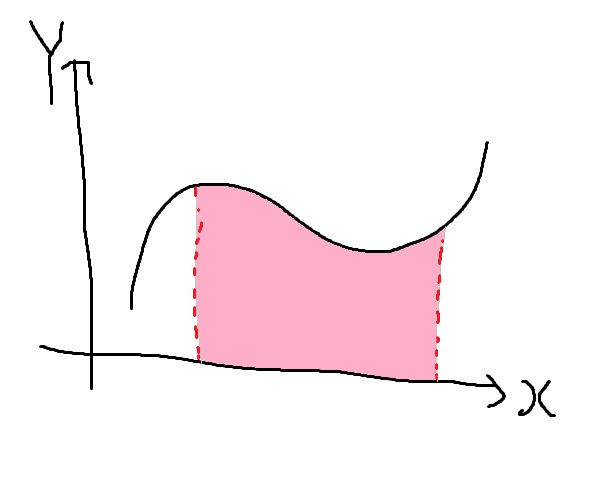
\includegraphics[width = 6cm]{area_under_graph.jpg}
\end{figure}


Our final total goodness function becomes:
\[ \text{Goodness}(T) = \int_{t_\text{start}}^{T} \text{tastiness}(t) \,\dx[t] + \text{tastiness}(T) \]
We will finish this off next time.
\finishEntry{}